%!TEX root = ../dissertation.tex
% this file is called up by thesis.tex
% content in this file will be fed into the main document

\graphicspath{{7-timbre/figures/}}

\chapter{Synthesizer-Aided Multi-Instrument Transcription}
\label{ch:timbre}

Revisit the first chapter, collect the background 

In this chapter, ...

\section{Introduction}

multi-instrument transcription is a difficult problem

\section{Background}


\subsection{Multi-Instrument Music Transcription}

\cite{itoyama2011bayesian}: instrument recognition, \TODO{add more; interconnected with source separation}

\cite{grindlay2009eigeninstruments}: Hierarchical eigeninstruments

\cite{benetos2015probabilistic}: Probabilistic model (PLCA), spectral template, EM maximization

\cite{thickstun2017musicnet}: MusicNet, \cite{thickstun2018invariances} invariances,

\subsection{Deep Clustering}

\cite{hershey2016deepclustering}

\subsection{Source-Filter Synthesis}

\cite{heittola2009separation}

\subsection{Synthesizer Component for Transcription}

\citeA{li2017infinite} explored the idea of using on-the-fly synthesized training dataset for piano transcription, using a simple fully-connected neural network operating on the CQT representation.
The idea of using generative models to predict multiple fundamental frequencies is also not new \cite{dubois2005harmonic,cemgil2006generative}, but the authors relied on manually designed generative models for sound generation, which limits the expressibility and the generalizability of the model.
Using deep generative models can be a direction for overcoming these limitations, since the recent neural network approaches for audio generation are capable of producing highly realistic sounds.

\cite{choi2019drum}


\section{Method}

\subsection{Synthesizer Model}

\begin{figure}
	\centering
	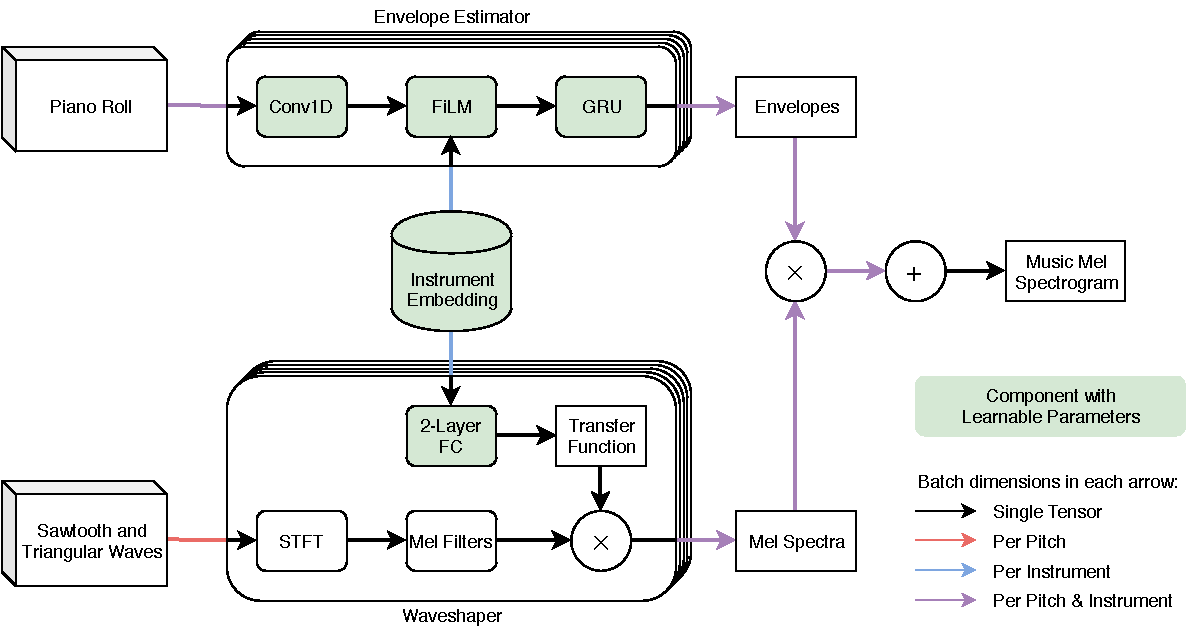
\includegraphics[width=\textwidth]{synthesizer-architecture.pdf}
	\caption{\TODO{write}}\label{fig:synthesizer-architecture}
\end{figure}


\subsection{Synthesizer as Regularizer}

\begin{itemize}
	\item unit-norm timbre embedding space
	\item complex Mel-based synthesizer
	\item polynomial-regression filter
	\item CRNN/FiLM-based ADSR
	
	\item tuning fix
\end{itemize}

\subsection{Tuning Correction}

\section{Experimental Setup}

\begin{itemize}
	\item dataset
	\item trained synthesizer
	\item with/without timbre embedding
	\item predicted/binarized vs GT frame labels
\end{itemize}

\section{Results}

\begin{itemize}
	\item Trained Synthesizer
	\item Transcription Metrics
	
\end{itemize}


\section{Conclusion}

\begin{itemize}
	\item Discussion points: unison, dot product space
\end{itemize}

